\section{Chameleon Framework: Generating Malicious, Evasive PDFs}
\label{ss: implementation}

Our study is based on various evasions, which we summarize in a taxonomy (Section~\ref{ss: evasions}).
To systematically study how these evasions evade malware scanners, we present Chameleon, a framework to automatically create malicious files that contain one or more evasions.
Our implementation of the framework focuses on malicious PDF documents.
Such malware is particularly interesting because document-based malware attacks are a prevailing problem~\cite{pdf_cve_statistics, officeonrise, exploit_CVE_2018_4990} and because the ability of PDF scanners to cope with evasions is currently understudied.

Figure~\ref{fig: chameleon overview} shows an overview of the Chameleon framework.
The inputs to the framework are a set of evasions, a set of \emph{exploits}, i.e., code 
that uses a bug or vulnerability, and a set of \emph{payloads}, i.e., code that contains the malicious behavior of the attack.
We discuss these inputs in Sections~\ref{ss: evasions}, \ref{ss: exploits}, and~\ref{ss: payloads}, respectively.
Given these inputs, Chameleon generates evasive PDF documents and validates that they still behave maliciously despite the evasion(s).
We then pass these documents to a set of PDF scanners (Section~\ref{ss: analyzers}) and measure their ability to handle the evasions (Section~\ref{ss: results}).

\begin{figure}
    \centering
    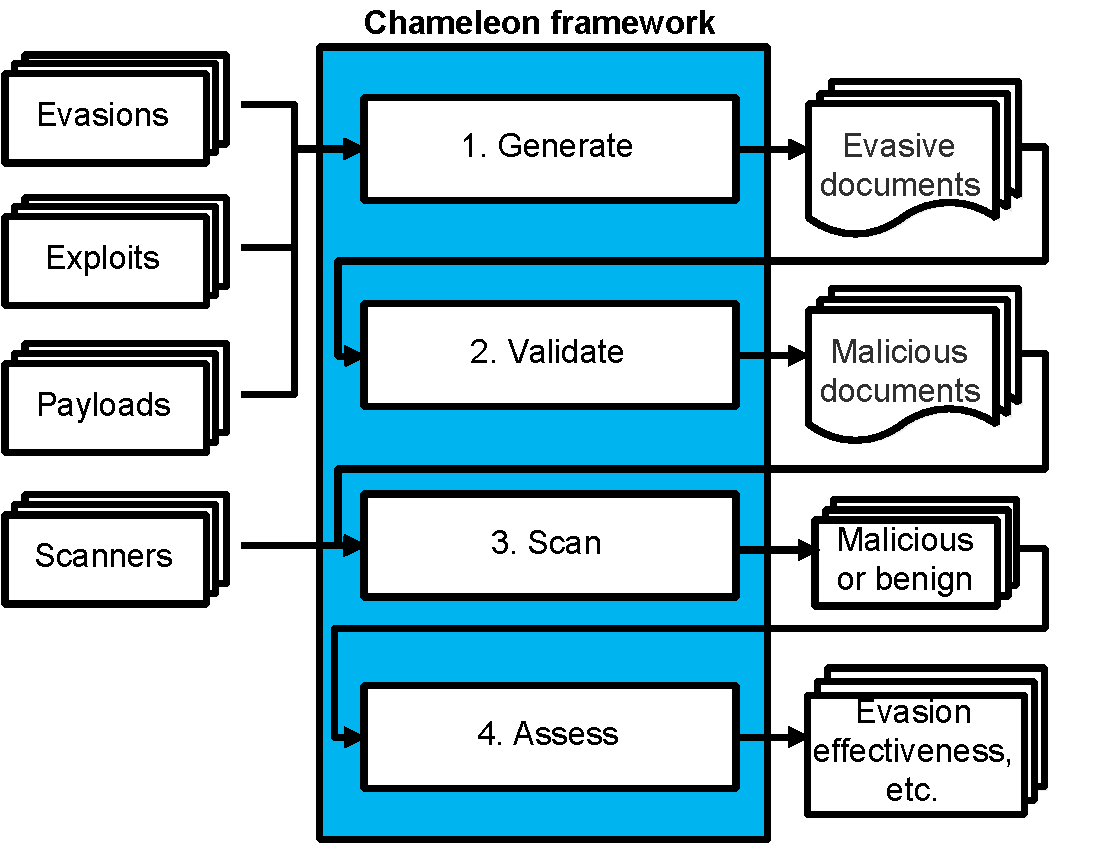
\includegraphics[width=0.5\textwidth]{figures/overview.pdf}
    \caption{Overview of the Chameleon framework and its four steps.}
    \label{fig: chameleon overview}
\end{figure}


\subsection{Evasions}
\label{ss: evasions}

Various evasion techniques, for executables and other potentially malicious
file formats have been proposed~\cite{corona2014lux0r,pdfstaticevasion,pdf_obfus_odd_algs,related_static_obfus,vmray_anti_evasion,joe_anti_evasion,lastline_anti_evasion,fireeye_anti_evasion}.
To provide some background on different kinds of evasions and the scope of this 
work, we present a taxonomy of evasions.
The taxonomy tries to cover the major classes of evasions that are relevant for 
malicious documents without claiming to be complete.
In particular, we focus on evasions implemented in high-level languages that 
can be embedded into document formats, such as JavaScript and Visual Basic.

\begin{figure*}[tb]
\small
\centering
\Tree 	[.{Evasions}
          [.Static
    				{Run-time \\ Loading}
    				Obfuscation
    			]
    			[.Dynamic 
    				[.Environment
    					Network {File System} Context Timing Architecture
    				]
            [.{UI} Human Machine ]
    				{Random \& \\ Time-based}
          ] ]
\captionsetup{justification=centering}
\caption{A taxonomy of evasion techniques.}
\label{f:taxonomy}
\end{figure*}

Figure~\ref{f:taxonomy} shows an overview of the taxonomy.
We distinguish between dynamic and static evasions.
\emph{Static evasions} attempt to modify the document or the code embedded 
into it in a way that influences a static analysis of the document.
In contrast, \emph{dynamic evasions} change the run-time behavior of a 
document to influence the outcome of a dynamic analysis of the document.

\subsubsection{Static Evasions}
Among the static evasions, there are two broad classes.
First, \emph{run-time loading} tries to conceal malicious behavior by loading 
parts of the code at run-time, making it harder for a static scanner to 
detect the maliciousness.
For example, an evasion based on run-time loading may download the malicious 
payload once the document is opened on the victim's machine, i.e., after 
having been checked by a static scanner.
Second, \emph{obfuscation} modifies the malicious source code to conceal its 
purpose.
There are various obfuscation techniques, such as encryption, multi-pass 
encoding, logical xor, and changing the code 
structure~\cite{pdfstaticevasion}.

\subsubsection{Dynamic Evasions}
Dynamic evasions can be broadly classified into three categories.
The first category are \emph{environment-based evasions}, which attempt to 
take the execution environment into account.
This approach is specially appealing for targeted attacks, where the 
attacker has some information about the target system. We further classify environment-based evasions 
into the following five categories:

\textbf{Network}.
    Dynamic scanners may restrict the network access of documents to prevent malware from downloading its payload.
    Network-based evasions check the network connection to identify the 
    presence of a dynamic scanner or a sandbox.
  
\textbf{File system}.
    Since many dynamic scanners rely on known libraries or executables, the 
    presence of particular files in the file system may disclose a dynamic 
    scanner.
    File system-based evasions check whether particular files exist to 
    decide whether to perform any malicious behavior.

\textbf{Context}.
    Information about the system language, locales, most recently used 
    documents, the time zone, etc.\ can be abused by attackers to target 
    particular victim systems~\cite{le2017broad, rasthofer2017making}.
    A context-based evasion deceives dynamic scanners by behaving 
    maliciously only in particular contexts.

\textbf{Timing}.
    Due to the virtualized environment used by most dynamic scanners, some 
    operations have observably lower performance than other operations.
    For example, the performance difference of a CPU-intensive computation
    and a GPU-intensive computation is higher in a virtual machine than on a 
    physical machine.
    The reason is that in a modern virtual machine, many CPU instructions 
    run natively, whereas translating GPU instructions to physical 
    instructions imposes a noticeable overhead~\cite{ho2014tick}.
    Timing-based evasions exploit such differences in execution time to 
    determine the presence of a dynamic scanner~\cite{timing_evasion}.
    
\textbf{Architecture}.
  These  evasions recognize architectural idiosyncrasies of the 
    underlying physical or virtual machine.
    Examples include an incorrectly return value of the \code{CPUID} instruction in
    QEMU~\cite{ferrie2007attacks} and GPU fingerprinting~\cite{gpufingerprinting}.

\medskip
The second category of dynamic evasions are \emph{UI-based evasions}.
Such evasions monitor interactions with UI elements to determine whether a 
human or a machine is using the system.
We further classify UI-based evasions into two sub-classes:

\textbf{Human user}.
    These evasions attempt to identify a human user and expose the 
    malicious behavior only to such users.
    For example, an evasion may wait until the user scrolls to a 
    particular page or clicks a particular UI 
    element~\cite{userinteraction}.

\textbf{Machine user}.
    Instead of trying to detect a human user, an evasion may also check for 
    evidences that a machine is interacting with the system.
    For example, text entered into a form with a superhuman 
    typing speed or clicks on an invisible element suggests the presence of a machine 
    user~\cite{keragala2016detecting}.

\medskip
The third category of dynamic evasions are \emph{random-based and time-based 
evasions}.
This kind of evasion triggers an attack either probabilistically or 
depending on the current time, e.g., only on specific times of the 
day~\cite{timebased}.


\subsubsection{Implementation of Evasions}
\label{ss: combination of evasions}

\begin{table*}[t]
\caption{Static and dynamic evasions implemented in the Chameleon framework. The last column denotes whether the evasion is implemented in the PDF structure, the embedded JavaScript code, or both.}
\label{t:evasions}
\footnotesize
\begin{tabular}{@{}p{6em}p{6em}p{39em}p{7.5em}@{}}
\toprule
Class & Name & Description & Implementation\\
\midrule
\multicolumn{3}{l}{\emph{Static evasions:}} \\
\midrule

Run-time loading & steganography & Encode the JavaScript code into 
                          an image file embedded in the PDF document. Load 
                          and \code{eval} the code at run-time. & PDF \& JavaScript \\

                          & content & Store the JavaScript code as the content in the 
                        PDF document. Load and \code{eval} the code at run-time. & PDF \& JavaScript \\
\\
JavaScript \mbox{obfuscation} & rev & Lexically reverse the JavaScript code. & JavaScript  \\

                          & xor & Encode the JavaScript code by applying 
                        the bitwise xor operator with the specified key. & JavaScript \\
\\                        
PDF \mbox{obfuscation}    & objstm & Compress the malicious PDF as an Object 
                          Stream and put it into a benign PDF document. & PDF 
                          \\

                          & nest & Recursively embed the malicious PDF into 
                          a benign PDF document for one or more times. & PDF                       
                          \\
                        & decoy & Insert the malicious JavaScript code 
                        into a benign PDF document. In contrast  to ``nest'', this evasion does not recursively nest documents into each other. & PDF
                        \\

\midrule 
\multicolumn{3}{l}{\emph{Dynamic evasions:}}\\
\midrule 
Context               & lang & Trigger if the language of the PDF viewer 
is in the specified set of languages. & JavaScript \\

                          & resol & Trigger if the desktop resolution is 
                          in the specified range. & JavaScript \\
                          
                          & mons & Trigger if the user's computer has the specified 
                          number of monitors attached to it. & JavaScript  \\

                          & filename & Trigger if the generated exploit's 
                          filename has not changed. Some scanners change the filename before the analysis. & JavaScript \\

\\
UI                        & scroll & Trigger when the user has scrolled 
                            to the specified page. & PDF \\

                            & captcha & Trigger if the user's text 
                            input matches the specified string. & JavaScript \\
                            
                            & alert\_three & Show an alert dialog box with 
                            three buttons and trigger if the specified                       
                            button is clicked. & JavaScript \\
                
                            & doc\_close & Trigger when the document gets 
                            closed. & PDF  \\
                            
                            & alert\_one & Show an alert dialog box with one                                
button and trigger when the button is clicked. & JavaScript \\
                            
                            & mouse & Trigger if the mouse position 
                            changes. & JavaScript \\
\\
Random and time-based   & delay & Delay the exploitation for the                                
given amount of time (time bomb). & JavaScript \\

                            & tod & Trigger at the specified time of the day. & JavaScript  
                            \\

\bottomrule
\end{tabular}
\end{table*}

Based on our taxonomy, we have implemented 19 evasions (7 static and 12 dynamic), as summarized in Table~\ref{t:evasions}.
Some evasions take an argument to configure different variants of the evasion.
For example, the ``lang'' evasion can be configured by passing the language to check for, and the ``delay'' evasion can be configured with a specific amount of time.
Using the ``lang'' evasion with ``English'' as the argument will result in a document that attacks only computers with the English version of Adobe Reader:
{\tt \small
\begin{verbatim}
if (app.language == "English")
  exploit(); // trigger the exploit
\end{verbatim}
}

In addition to injecting individual evasions into documents, Chameleon 
also allows to  blend multiple evasions into \emph{combined evasions}.
We refer to combined evasions that contain at least one static and at least 
one dynamic evasion as \emph{hybrid evasions}.
When combining evasions of the same kind, we focus on evasions from different classes, e.g., run-time loading with JavaScript obfuscation.
For UI-based evasions, we also combine several evasions from the same class to gradually increase the complexity of the UI interactions required to trigger the attack.
Moreover, Chameleon creates an evasion that combines several context-based evasions, to create a document that targets a very specific environment and remains silent otherwise.

\subsection{Exploits}
\label{ss: exploits}

Chameleon uses two PDF exploit modules provided by the Metasploit framework\footnote{\url{https://github.com/rapid7/metasploit-framework}} and adapts them to introduce evasions.
The ``Toolbutton'' exploit\footnote{CVE-2013-3346} abuses a use-after-free vulnerability in the implementation of the Adobe-specific JavaScript function \code{app.add\-Tool\-Button}.
The exploit executes some JavaScript code to set up the environment and then triggers the vulnerability by calling the vulnerable function.
To implement dynamic evasions, we trigger the vulnerability only if the condition checked by the evasion holds.

The ``Cooltype'' exploit\footnote{CVE-2010-2883} uses a malicious font file in addition to malicious JavaScript code.
The font file is loaded after the JavaScript code has set up the environment for exploitation.
We slightly modify the exploit by adding an exploitation trigger that controls whether and when the exploit is executed.
The dynamic evasions call this trigger only if the condition checked by evasion holds.

In addition to ``Toolbutton'' and ``Cooltype'', Metasploit provides other PDF exploit modules.
We choose these two exploits as they target a popular PDF reader software (Adobe Reader) and because
they are old and well-known. If our evasions can fool PDF scanners using old and well-studied
exploits then the evasions are at least as or even more effective when applied to more recent
or zero-day exploits.

\subsection{Payloads}
\label{ss: payloads}

Another important component of any attack is the payload that it carries.
As payloads, Chameleon uses native machine code that is executed after the vulnerability is triggered.
We use three different payloads, two provided by Metasploit and one that we develop ourselves.
The first payload, ``Reverse Bind'', establishes a TCP connection to a remote host allowing the remote host to control the exploited machine.
The second payload, ``Powershell'', spawns an instance of Windows Powershell with a command that creates a text file in a temporary directory.
The third payload, ``Exit'', simply exits the Adobe Reader process.

\subsection{Generating and Validating Evasive Documents}

We implement the Generate step of Chameleon on top of the Metasploit framework, which we use to generate exploit documents, and the Origami PDF transformation library\footnote{\url{https://github.com/gdelugre/origami}}, which we use to manipulate documents.
The 19 evasions are implemented as a new Metasploit module, which can be used with any of the PDF exploit modules.

After generating a supposedly malicious document, Chameleon checks that the document is indeed malicious (step Validate).
To this end, Chameleon opens the document in the vulnerable version of Adobe Reader inside a sandbox, interacts with it according to the evasions (e.g., by moving the mouse or waiting for some time), and checks whether the payload is executed.
At the moment this process is mostly but not fully automated because for context-based evasions, the sandbox needs to be manually adapted to the context that an evasion is looking for (e.g., for the ``mons'' evasion, the number of displays attached to the sandbox has to be properly set).

Our implementation and a set of \nbSamplesSize{} generated PDF documents are publicly available.\footnote{\url{https://github.com/sola-da/Chameleon/}}
